\section{Verifica}
Per verifica si intende l'insieme delle attività volte a garantire che il prodotto \textit{software} sviluppato soddisfi i requisiti specificati e funzioni correttamente in tutte le condizioni previste. Non si tratta quindi soltanto di individuare errori, ma di adottare un approccio disciplinato che assicuri qualità, affidabilità e coerenza con le specifiche.  

In questo progetto, le attività di verifica seguono metodologie consolidate dell'ingegneria del \textit{software}, in particolare lo \textbf{schema a V} e lo sviluppo guidato dai \textit{test} \gls{tdd}. L'adozione di tali metodologie ha permesso di strutturare in maniera rigorosa l'intero processo, dalla fase di analisi fino al collaudo, garantendo tracciabilità e coerenza tra fasi di sviluppo e attività di verifica.  

\subsection*{Schema a V}
Abbiamo adottato lo schema a V (Figura~\ref{fig:schema-v}) come riferimento metodologico per pianificare e coordinare le attività di sviluppo e verifica.\\
In particolare, i requisiti funzionali sono messi in relazione con i \textit{test} di accettazione, volti a garantire che le funzionalità implementate rispondano correttamente alle esigenze espresse.\\
I requisiti non funzionali sono rappresentati dai \textit{test} di sistema, che hanno permesso di validare aspetti quali prestazioni, sicurezza, usabilità e scalabilità.\\
I requisiti di vincolo sono associati ai \textit{test} di conformità, necessari ad assicurare l'aderenza a \textit{standard}, normative e specifiche tecniche.\\
Per quanto riguarda le fasi progettuali, la progettazione architetturale ha ricevuto la verifica tramite \textit{test} di integrazione, mentre la progettazione di dettaglio ha trovato corrispondenza nei \textit{test} unitari, volti al controllo puntuale di ogni singola funzione o metodo.


Questa impostazione ha garantito una verifica progressiva e multilivello, con una copertura completa dalla macro-struttura fino al singolo metodo.  

\begin{figure}[H]
    \begin{center}
    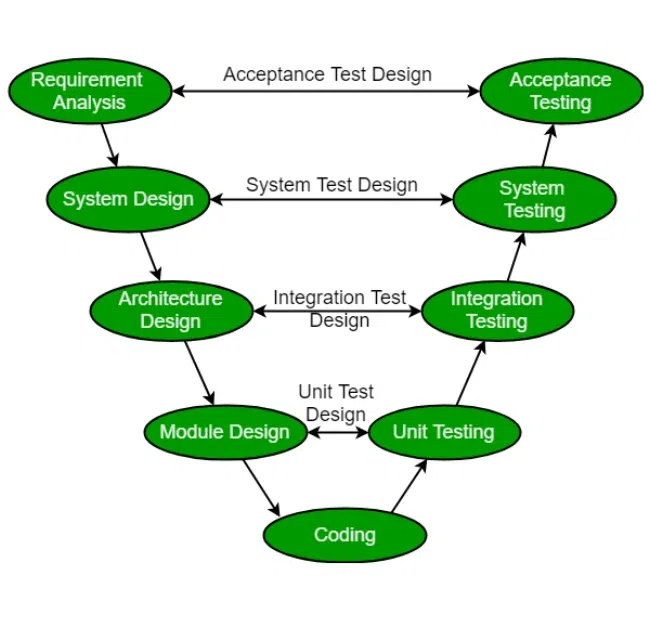
\includegraphics[width=0.8\textwidth]{img/V-model.png}
    \caption{Rappresentazione dello schema a V adottato nel progetto.}
    Fonte: \url{https://www.geeksforgeeks.org/software-engineering/software-engineering-sdlc-v-model/}
    \label{fig:schema-v}
    \end{center}
\end{figure}

\subsection*{Test-Driven Development (TDD)}
Parallelamente, ho adottato la metodologia \textit{TDD}, che ha guidato l'implementazione del codice attraverso cicli iterativi caratterizzati dalle tre fasi classiche:
\begin{enumerate}
    \item \textit{\textbf{Red}}: scrittura del \textit{test} relativo a una nuova funzionalità, inizialmente fallito;
    \item \textit{\textbf{Green}}: implementazione della funzionalità per soddisfare il \textit{test};
    \item \textit{\textbf{Refactor}}: miglioramento del codice, mantenendo il superamento dei \textit{test}.
\end{enumerate}
Questo approccio ha favorito lo sviluppo di codice modulare, riusabile e più semplice da mantenere, riducendo la probabilità di introdurre errori nelle fasi successive.  

\begin{figure}[H]
    \begin{center}
    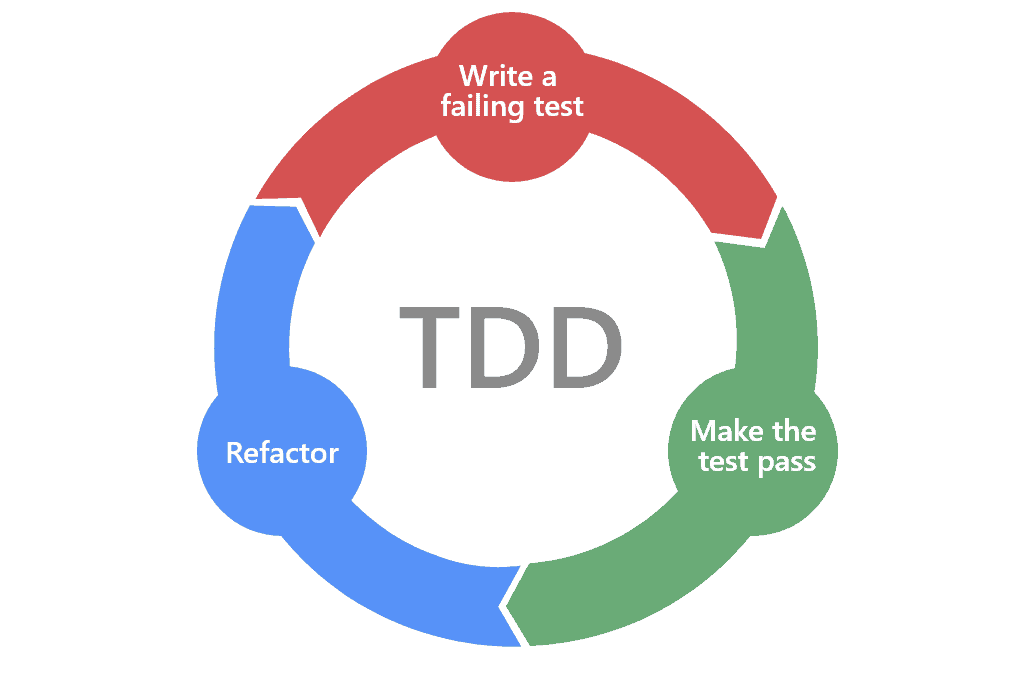
\includegraphics[width=0.9\textwidth]{img/TDD.png}
    \caption{Schema del ciclo TDD utilizzato durante lo sviluppo.}
    Fonte: \url{https://marsner.com/blog/why-test-driven-development-tdd/}
    \label{fig:tdd}
    \end{center}
\end{figure}

\subsection{Test e strumenti}
I \textit{test} li ho scritti utilizzando la libreria \textit{pytest}, che consente di scrivere casi di \textit{test} in modo semplice e leggibile. Per aumentare l'efficacia della verifica, ho utilizzato librerie complementari quali:
\begin{itemize}
    \item \textit{pytest-mock}, per la simulazione di oggetti e funzioni;
    \item \textit{pytest-cov}, per il calcolo della copertura del codice.
\end{itemize}

Sono presenti \textit{test} unitari per ogni funzione e metodo del progetto, con particolare attenzione a:
\begin{itemize}
    \item casi normali, per validare il comportamento atteso;
    \item casi limite, per testare condizioni particolari e scenari estremi;
    \item casi di errore, per valutare la robustezza e la gestione delle eccezioni.
\end{itemize}

\subsection{Risultati quantitativi}
Il processo di \textit{testing} ha prodotto risultati significativi in termini di completezza e profondità delle verifiche svolte:
\begin{itemize}
    \item l'implementazione di 94 test unitari e di integrazione;
    \item la copertura del codice ha raggiunto il 98\% (Figura~\ref{fig:coverage});
    \item l'identificazione e correzione di 5 \textit{bug} durante le iterazioni di \textit{TDD}, con una riduzione progressiva degli errori riscontrati nelle fasi avanzate.
\end{itemize}
Tali risultati dimostrano l'efficacia della strategia di verifica adottata e l'intensità del lavoro svolto per garantire la qualità del prodotto finale.  

\begin{center}
\begin{longtable}{|p{0.25\textwidth}|p{0.15\textwidth}|p{0.25\textwidth}|p{0.2\textwidth}|}
\hline
\multicolumn{1}{|c|}{\textbf{Tipo di test}} & 
\multicolumn{1}{c|}{\textbf{Quantità}} & 
\multicolumn{1}{c|}{\textbf{Copertura}} & 
\multicolumn{1}{c|}{\textbf{Durata esecuzione}} \\ 
\hline
\endfirsthead

\multicolumn{4}{c}{{\bfseries \tablename\ \thetable{} -- Continuo della tabella}}\\
\hline
\multicolumn{4}{|c|}{\textbf{Attività di testing quantificate}} \\ \hline
\endhead

\hline \multicolumn{4}{|r|}{{Continua nella prossima pagina...}} \\ \hline
\endfoot

\endlastfoot

Test unitari & 78 & 98\% componenti & 14.5 secondi \\ \hline
Test di integrazione & 16 & 100\% componenti & 3.7 secondi \\ \hline
\textbf{TOTALE} & 94 & 98\% globale & 18.2 secondi \\ \hline

\caption{Tabella quantitativa delle attività di \textit{testing}.}
\label{tab:attivita-testing}
\end{longtable}
\end{center}

\begin{center}
\begin{longtable}{|p{0.18\textwidth}|p{0.1\textwidth}|p{0.15\textwidth}|p{0.1\textwidth}|}
\hline
\multicolumn{1}{|c|}{\textbf{Categoria}} & 
\multicolumn{1}{c|}{\textbf{Numero bug}} & 
\multicolumn{1}{c|}{\textbf{Severità media}} & 
\multicolumn{1}{c|}{\textbf{Tempo medio risoluzione}} \\ 
\hline
\endfirsthead

\multicolumn{4}{c}{{\bfseries \tablename\ \thetable{} -- Continuo della tabella}}\\
\hline
\multicolumn{4}{|c|}{\textbf{Bug rilevati e metriche di risoluzione}} \\ \hline
\endhead

\hline \multicolumn{4}{|r|}{{Continua nella prossima pagina...}} \\ \hline
\endfoot

\endlastfoot

\textit{Parser regex} & 3 & Media & 8 ore \\ \hline
\textit{Container} & 2 & Alta & 16 ore \\ \hline
\textbf{TOTALE} & 5 & Media-Alta & 24 ore \\ \hline

\caption{Tabella quantitativa dei bug rilevati e del tempo di risoluzione medio.}
\label{tab:bug-metriche}
\end{longtable}
\end{center}


\begin{figure}[H]
    \begin{center}
    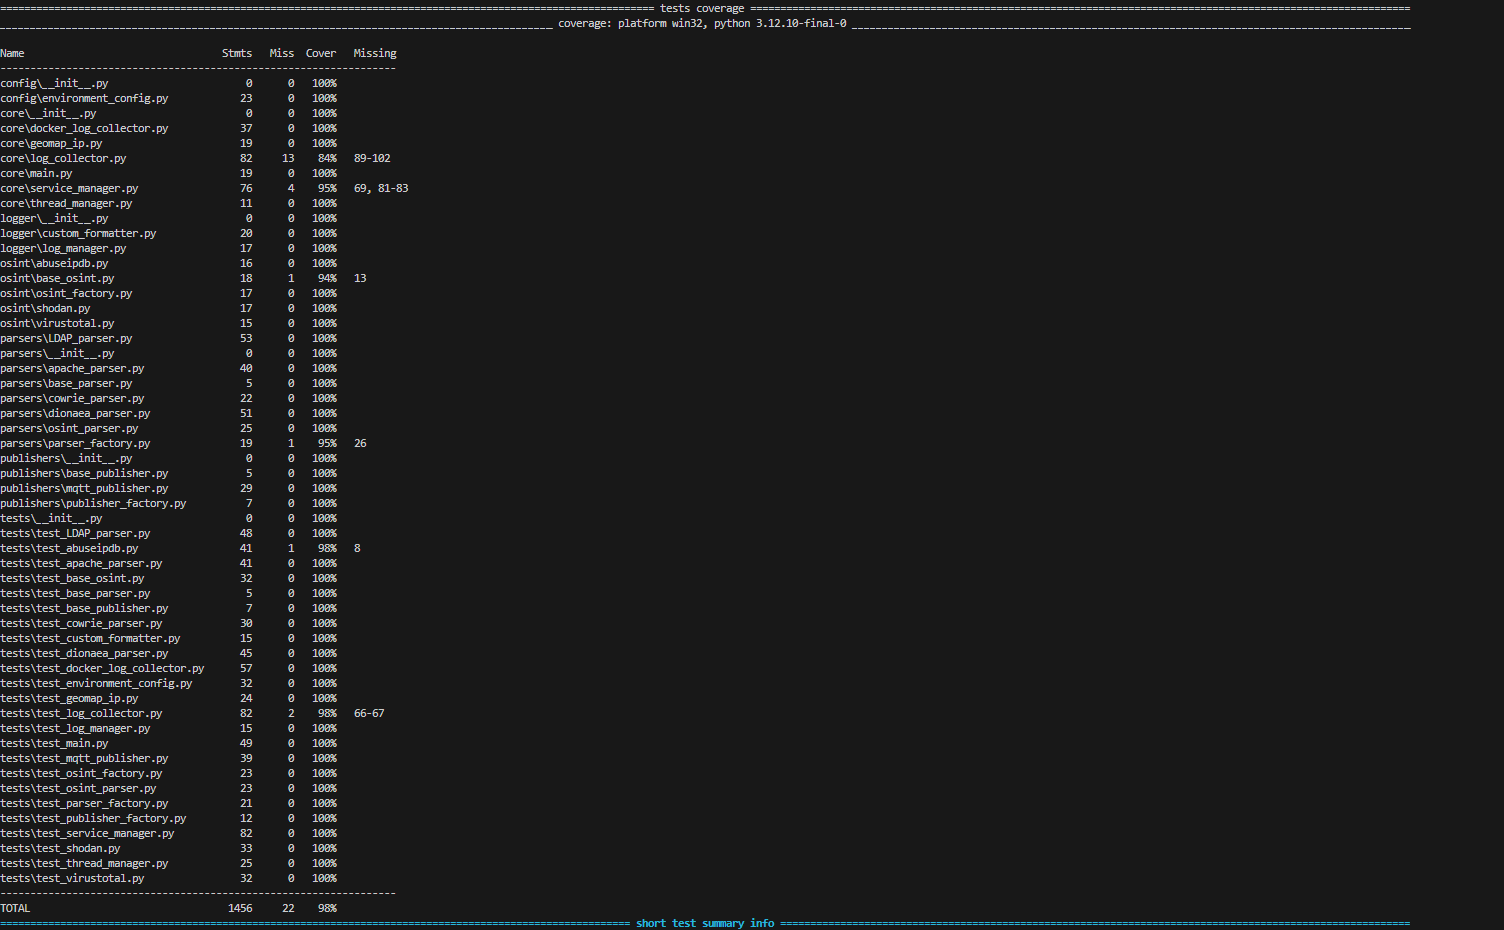
\includegraphics[width=\textwidth]{img/code-coverage.png}
    \caption{Risultato della copertura del codice dopo l'esecuzione dei \textit{test}.}
    \label{fig:coverage}
    \end{center}
\end{figure}
